\documentclass[10pt,twocolumn]{article}
\usepackage[margin=0.72in]{geometry}
\usepackage{amsmath,amssymb,booktabs,graphicx,microtype,url}
\usepackage[hidelinks]{hyperref}
\title{Spatiotemporal Detection and Localized Suppression\\of Rapid Visual Changes in Video}
\author{Undergraduate Computer Vision Research Project}
\date{September 2026}
\begin{document}
\maketitle

\begin{abstract}
This work asks whether spatially localized temporal filtering can reduce rapid brightness changes while preserving unaffected image regions better than whole-frame filtering. We implement interpretable global and block baselines, then develop an event-specific adaptive candidate that separates opposing luminance transitions, saturated-red transitions, and regular high-contrast patterns. Each evidence channel receives a corresponding local correction: luminance-step limiting, desaturation, or contrast reduction. A deterministic ten-scenario synthetic benchmark evaluates the baselines, while a 47-second excerpt from an official lyric video provides a real-media case study for the adaptive candidate. On that excerpt, mean normalized temporal activity decreases from 0.06293 to 0.01408, although peak activity decreases only from 0.11880 to 0.11285 and visible alteration remains a quality tradeoff. Scene cuts and moving objects remain important confounds. These measurements are computational proxies, not clinical validation or a guarantee of seizure safety or standards compliance.
\end{abstract}

\section{Introduction}
Rapid changes in video can be spatially global, such as alternating full frames, or confined to a small object. A detector that averages the entire image can miss a small intense region; a global filter can also distort pixels unrelated to the detected event. This project studies the resulting suppression--preservation tradeoff with transparent algorithms suitable for inspection and modification by a student.

The contribution is an end-to-end reproducible testbed: explicit color handling, global and localized baselines, separable luminance/red/pattern evidence, event-specific corrections, ten deterministic synthetic cases with ground truth, a real-media case study, joint metrics, ablations, a command-line interface, and analytic tests. It does not model viewing distance, calibrated display luminance, or individual physiology. Consequently, its activity metric and analyzer outputs must not be interpreted as medical-risk measures.

\section{Related Work}
Accessibility guidance treats flash frequency, brightness/color transitions, and affected area as jointly relevant \cite{w3c2023flashes}. The present work is only inspired by the observation that area matters; its threshold is not a WCAG threshold and it performs no conformance assessment. ITU-R BT.709 specifies HDTV colorimetry \cite{itu709}; we use its RGB-to-luminance coefficients after explicitly inverting the sRGB transfer function.

General luminance flashes and transitions involving saturated red are treated as distinct cases in accessibility guidance \cite{w3c2023flashes}. Consequently, converting an entire video to grayscale is not a general solution: a luminance-preserving grayscale transform leaves black--white temporal differences essentially unchanged. We instead use desaturation only where the saturated-red proxy supplies evidence, while handling general flashes through a luminance-domain constraint.

Nomura et al. proposed an adaptive temporal filter driven by a model-derived index and evaluated it with photosensitive patients \cite{nomura2000adaptive}. Our system is not a reproduction of that clinical work. It instead uses a deliberately simpler signal-processing proxy and synthetic evaluation so every decision can be explained. We make no novelty or clinical-efficacy claim.

\section{Problem Formulation}
A video is $V=\{I_0,\ldots,I_{T-1}\}$ with $I_t\in[0,1]^{H\times W\times3}$. For an sRGB channel $C$, linearization is
\begin{equation}
C_{\mathrm{lin}}=\begin{cases}C/12.92&C\leq0.04045\\((C+0.055)/1.055)^{2.4}&\text{otherwise.}\end{cases}
\end{equation}
Relative luminance is $Y=0.2126R_{\mathrm{lin}}+0.7152G_{\mathrm{lin}}+0.0722B_{\mathrm{lin}}$. We compute
\begin{equation}
\Delta_t(x,y)=|Y_t(x,y)-Y_{t-1}(x,y)|,\quad D_t=\frac{1}{HW}\sum_{x,y}\Delta_t(x,y).
\end{equation}
If fraction $p$ of pixels change by magnitude $a$, then $D_t=pa$: spatial averaging dilutes small regions. Conceptually, filtering seeks
\begin{equation}
\min_{\widehat V}\mathcal{D}(V,\widehat V)\quad\text{s.t.}\quad\mathcal{R}(\widehat V)\leq\tau,
\end{equation}
where $\mathcal{D}$ is visual distortion and $\mathcal{R}$ is our defined activity proxy, not a medically validated risk function.

\section{Method}
\textbf{Global baseline.} If $D_t\geq\tau$, every pixel is blended toward the prior filtered frame: $\widehat I_t=(1-\alpha)I_t+\alpha\widehat I_{t-1}$. Otherwise, $I_t$ is retained.

\textbf{Localization.} Difference maps are averaged over the latest $w$ frames. The image is divided into $b\times b$ blocks, and every pixel in a block is selected when its mean activity exceeds $\tau$. An optional morphological closing fills small gaps. Gaussian smoothing converts the binary decision $B_t$ to a soft mask $M_t\in[0,1]$, reducing hard-boundary artifacts. The output is
\begin{equation}
\widehat I_t=(1-\alpha M_t)\odot I_t+\alpha M_t\odot\widehat I_{t-1}.
\end{equation}
Defaults are $\tau=0.12$, $b=8$, $w=2$, $\alpha=0.65$, closing width 3, and Gaussian $\sigma=2$. These are experimental choices, not safety limits. Processing is $O(THW)$ time and, in the current batch implementation, $O(THW)$ memory. Blocks were chosen over learned segmentation for interpretability; their main limitation is coarse boundaries.

\textbf{Separable event analyzers.} For the adaptive candidate, a flash pixel requires consecutive above-threshold transitions with opposite signs at the same location. Luminance evidence uses signed changes $L_t=Y_t-Y_{t-1}$. A simple, explicitly approximate red signal is
\begin{equation}
S_t=\begin{cases}R_t-\max(G_t,B_t),&R_t/(R_t+G_t+B_t)\geq0.8,\\0,&\text{otherwise,}\end{cases}
\end{equation}
and applies the same opposing-transition rule to $S_t-S_{t-1}$. This is not the complete WCAG chromaticity calculation. A separate $O(HW)$ tile detector finds approximately equally spaced alternating edges in horizontal or vertical mean profiles as evidence of regular high-contrast patterns. Gaussian smoothing feathers each spatial mask.

\textbf{Event-specific adaptive correction.} Let $M_t^L$, $M_t^R$, and $M_t^P$ denote soft luminance, red, and pattern masks. In $M_t^R$, the current color is blended toward an equal-channel grayscale value constructed from the same linear relative luminance. Thus chroma is reduced locally without claiming that grayscale addresses general flashing. In $M_t^L$, target luminance is clamped relative to the prior output:
\begin{equation}
Y_t^*=\operatorname{clip}(Y_t,\widehat Y_{t-1}-s,\widehat Y_{t-1}+s),
\end{equation}
then a neutral linear-RGB offset realizes the target before soft-mask compositing. This directly bounds detected luminance reversals and avoids the motion trails produced by recursive whole-region blending. In $M_t^P$, contrast is reduced around a Gaussian local mean $\mu_t$:
\begin{equation}
I_t^P=\mu_t+(1-\rho)(I_t-\mu_t).
\end{equation}
The three corrections remain independently configurable. Their default strengths are red desaturation $0.90$, luminance step $s=0.08$, and pattern contrast reduction $\rho=0.35$.

\section{Experimental Setup}
Ten 24-frame, $96\times64$ RGB sequences are generated with seed 7: whole-frame alternation; small, medium, multiple, and rapid localized alternation; static texture; gradual illumination; a scene cut; global exposure-like variation; and a moving bright object. The last five include negatives or confounds that a naive difference detector should handle poorly. Target cases provide per-frame masks.

Every method receives identical arrays. Activity measures include mean and peak $D_t$, threshold-exceeding frames, high-change area, and residual activity inside target masks. Distortion uses MAE, MSE, PSNR, and SSIM. We also report modified-pixel ratio, mask precision/recall/F1/IoU, elapsed time, and FPS. No-op similarity is perfect by construction, illustrating why distortion and suppression must be read jointly. Tests cover analytic luminance and activity cases, mask confusion counts, filter selectivity, lossless I/O, and a complete tiny benchmark.

For a real-media case study, we use a 47-second, $1280\times720$, 23.976-fps closing excerpt from the official lyric video for ``BREAK MY SOUL'' \cite{beyonce2022break}. This example was selected because its repeated large visual transitions make the suppression effect measurable; it is not labeled as medically hazardous. The diagnostic-strength adaptive configuration uses transition threshold 0.03, full red-event desaturation, luminance step $s=0.03$, pattern reduction $\rho=0.50$, and mask $\sigma=2$. Source and output are decoded together by \texttt{experiments/render\_frame\_differences.py}; the script writes the frame panels, plot, and JSON values used below.

\section{Results}
Table~\ref{tab:main} reports means across ten cases from the generated CSV. The localized method has the lowest mean and peak activity, but worse MAE and SSIM than the global baseline. Thus it does not dominate the baseline; it selects a different tradeoff.

\begin{table}[h]
\centering\small
\caption{Canonical benchmark means. Lower is better for activity, MAE, and modified area; higher is better for SSIM.}
\label{tab:main}
\begin{tabular}{lrrrrr}\toprule
Method & Mean & Peak & MAE & SSIM & Area\\\midrule
None & .1251 & .2007 & .0000 & 1.0000 & .0000\\
Global & .0385 & .1069 & .0403 & .9545 & .1386\\
Localized & .0356 & .0836 & .0449 & .9385 & .1562\\\bottomrule
\end{tabular}
\end{table}

For the small square, localization modifies 1.00\% of locations and achieves IoU 0.2623; its coarse block is larger than the labeled square. For whole-frame alternation it modifies 95.83\%, so localization provides no area advantage. Across target scenarios, IoU ranges from 0.2623 to 1.0000. The repository's generated tradeoff plot shows each per-case suppression--distortion pair and is derived directly from the same canonical CSV as Table~\ref{tab:main}.

\textbf{Real-media adaptive case study.} Table~\ref{tab:lyric} is generated from the paired lyric-video decoding. Mean activity falls by 77.6\%. At the strongest source transition (28.57 seconds), activity falls from 0.11880 to 0.02770; however, the maximum over the complete filtered excerpt is 0.11285 at a different frame. The latter result is important: reducing average activity does not guarantee elimination of every large transition. Mean absolute RGB modification is 0.08955, demonstrating that the diagnostic-strength configuration makes a substantial preservation tradeoff.

Figure~\ref{fig:lyric-frames} shows the actual adjacent decoded frames at the strongest source transition. The source changes from a nearly uniform red field to a nearly black field containing white text. The adaptive output retains the first frame but raises the second frame toward gray, reducing the corresponding luminance-difference map. This is also a clear example of the method's cost: the filtered current frame is visibly different from the source. Figure~\ref{fig:lyric-modification} isolates that modification and shows that this particular transition is essentially global rather than spatially localized.

\begin{table}[h]
\centering\small
\caption{Official lyric-video excerpt: normalized activity from the generated paired-video metrics.}
\label{tab:lyric}
\begin{tabular}{lrr}\toprule
Metric & Source & Adaptive\\\midrule
Mean activity & .06293 & .01408\\
Peak activity & .11880 & .11285\\
Activity at strongest source transition & .11880 & .02770\\\bottomrule
\end{tabular}
\end{table}

\IfFileExists{figures/lyric_adaptive/strongest_transition.png}{%
\begin{figure*}[t]
\centering
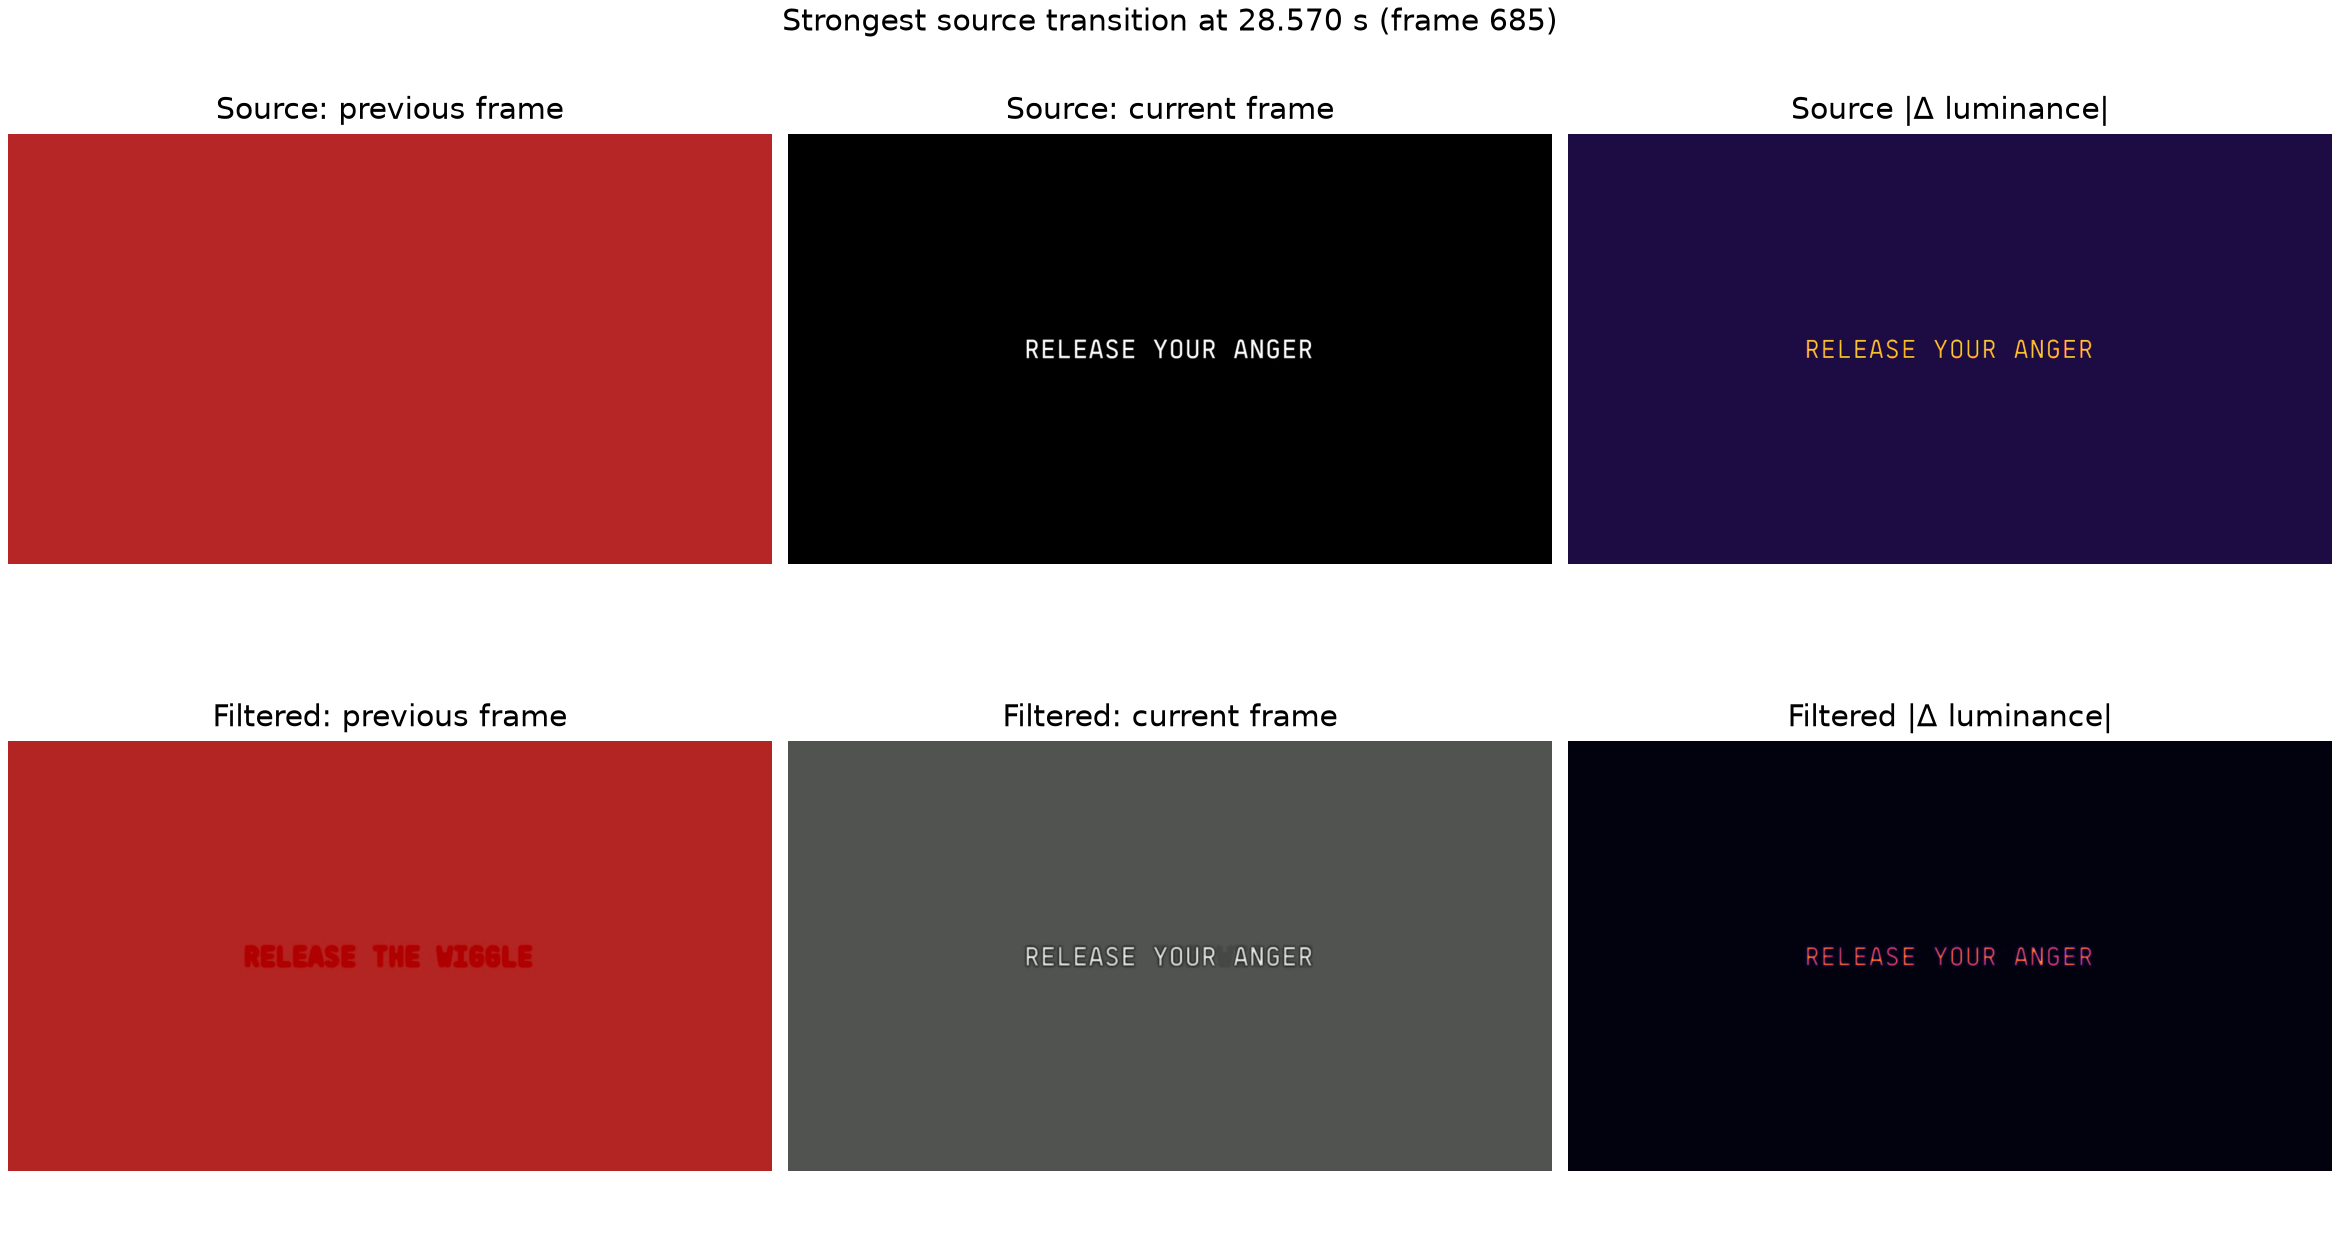
\includegraphics[width=.96\textwidth]{figures/lyric_adaptive/strongest_transition.png}
\caption{Actual adjacent frames at the strongest source transition in the lyric-video excerpt (28.57 seconds). Top: source previous frame, source current frame, and absolute relative-luminance change. Bottom: corresponding adaptive frames and change map. Heatmaps share the range $[0,1]$. The lower-right map is visibly weaker, but the gray filtered frame illustrates the associated appearance change. Frames are reproduced for research analysis from the official video \cite{beyonce2022break}.}
\label{fig:lyric-frames}
\end{figure*}%
}{}

\IfFileExists{figures/lyric_adaptive/source_filtered_difference.png}{%
\begin{figure*}[t]
\centering
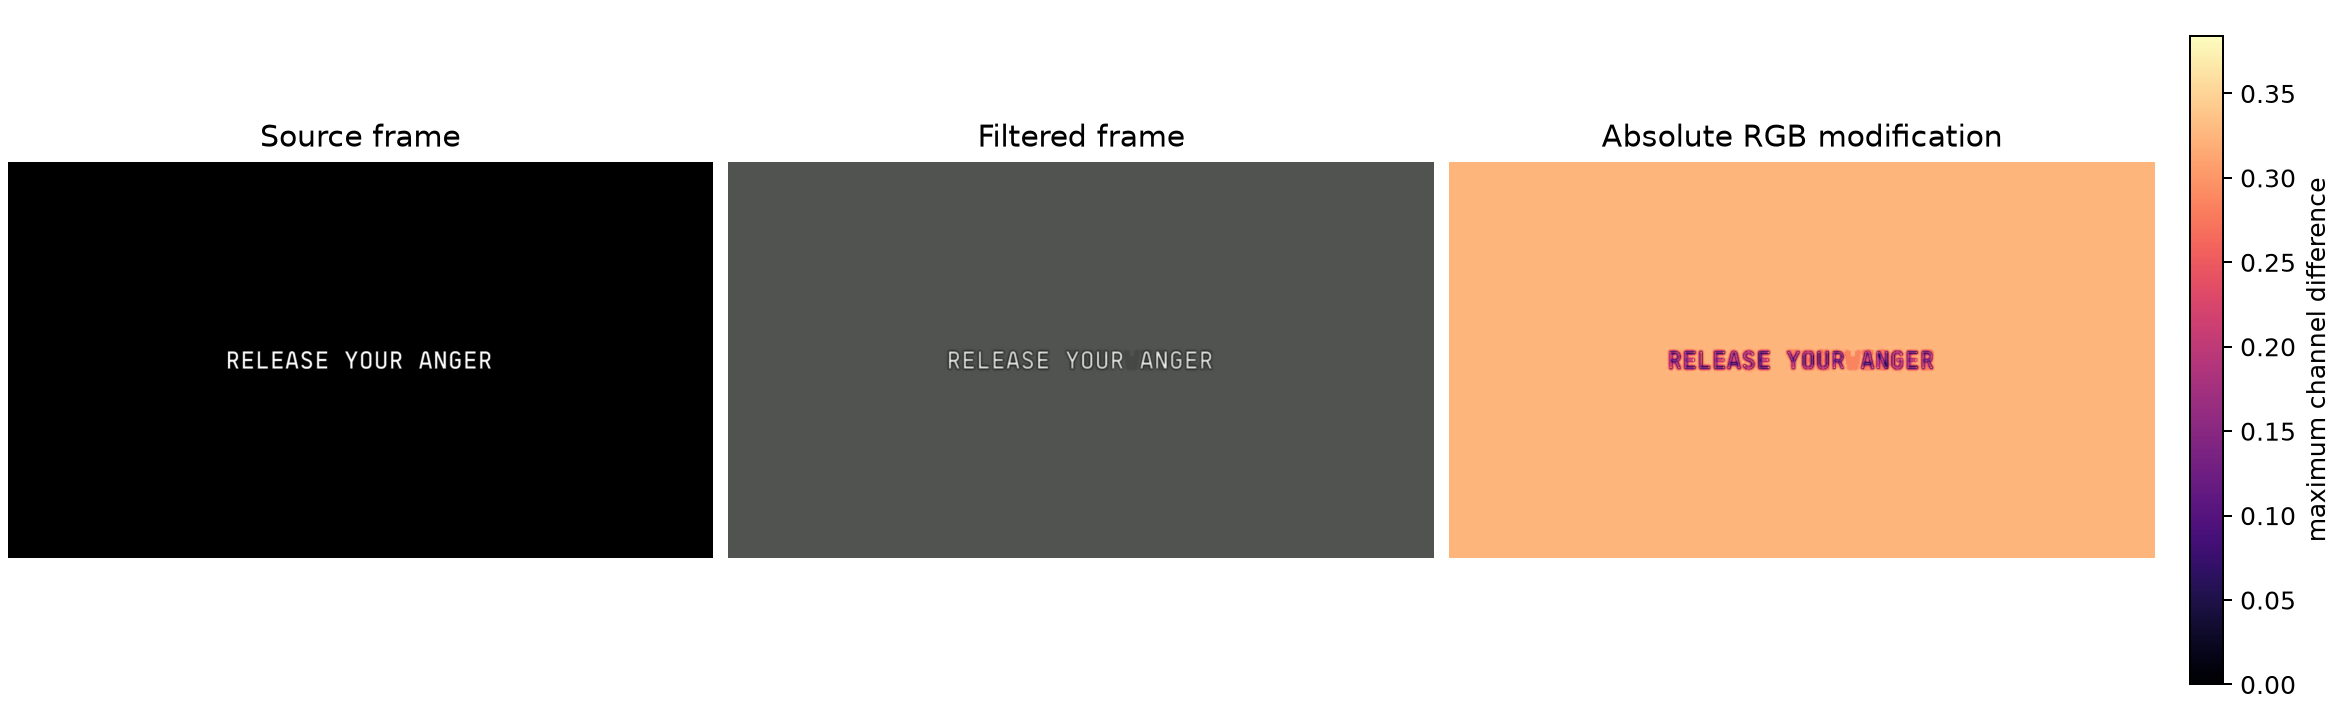
\includegraphics[width=.94\textwidth]{figures/lyric_adaptive/source_filtered_difference.png}
\caption{Source current frame, adaptive current frame, and per-pixel maximum absolute RGB-channel modification at the same transition. The nearly uniform modification map indicates that the detected event covers most of the frame; localization cannot preserve a large unaffected background in this example.}
\label{fig:lyric-modification}
\end{figure*}%
}{}

\IfFileExists{figures/lyric_adaptive/temporal_activity.png}{%
\begin{figure*}[t]
\centering
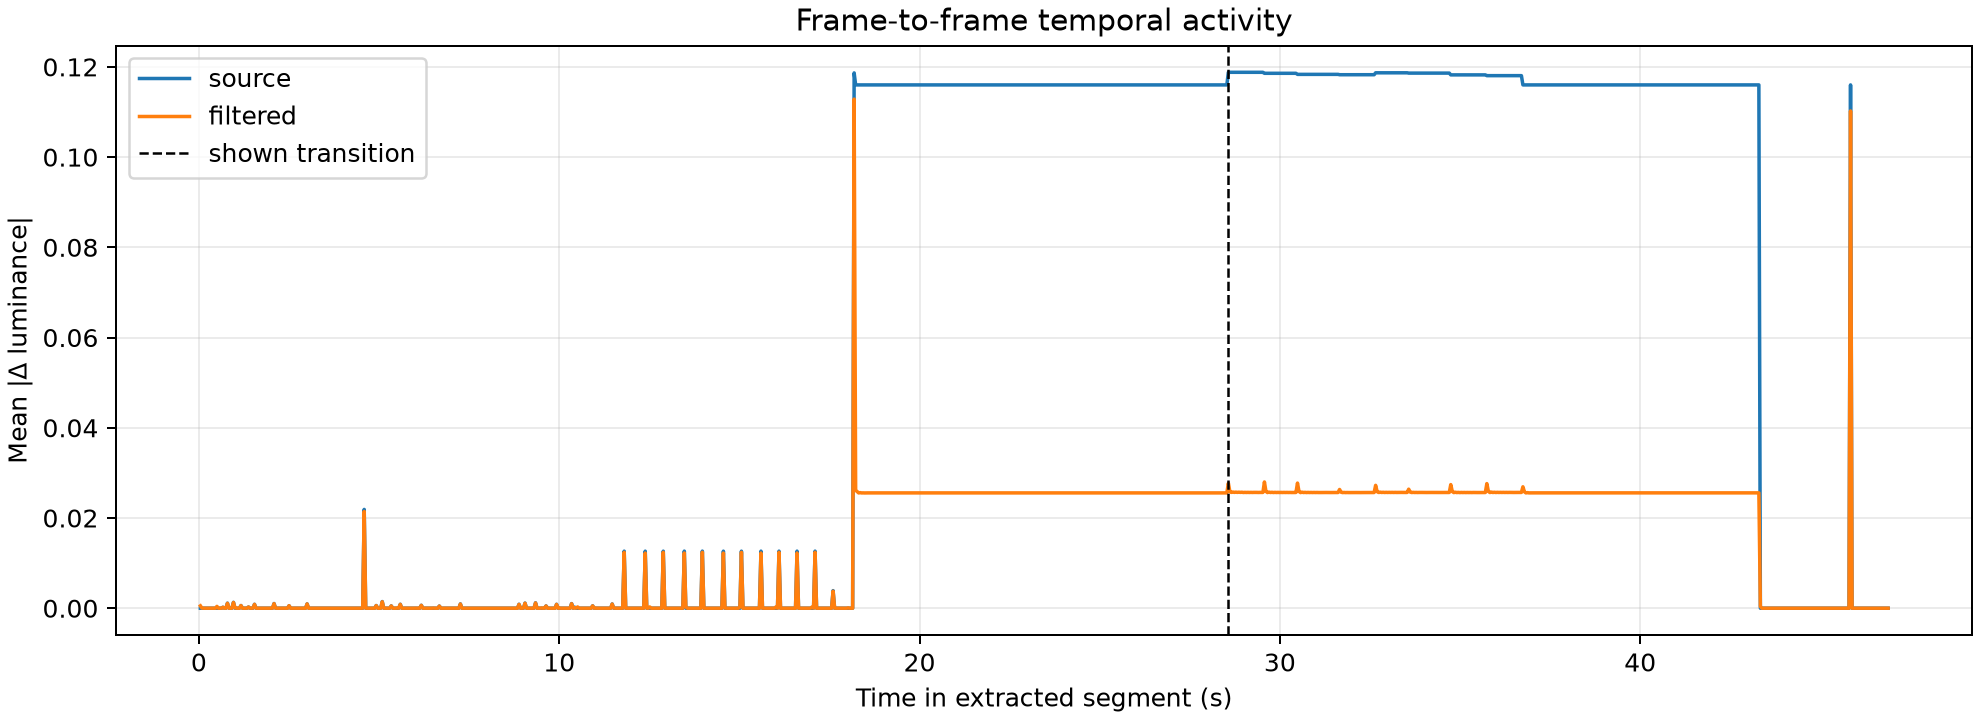
\includegraphics[width=.88\textwidth]{figures/lyric_adaptive/temporal_activity.png}
\caption{Temporal activity for the lyric-video excerpt. The adaptive output substantially lowers repeated activity across much of the segment, while isolated residual peaks remain. Generated directly from decoded source and filtered frames.}
\label{fig:lyric-activity}
\end{figure*}%
}{}

\section{Ablation Study}
The default localized configuration has mean IoU 0.6589 across all ten cases under the defined empty-mask convention. Reducing block size from 8 to 4 improves mean IoU to 0.7511 with nearly unchanged mean activity (0.0361), while block size 16 yields 0.6874. A hard mask reduces mean activity from 0.0356 to 0.0343 but raises MAE from 0.0449 to 0.0456 and may create seams. Morphological cleanup has no measurable effect on these clean shapes. Threshold 0.08 modifies more area (0.1648) than threshold 0.18 (0.1558). These results do not establish universal parameter choices.

\section{Failure Cases and Limitations}
The localized method modifies 8.33\% of locations at a scene cut and 2.11\% for a moving bright object; both have zero IoU against their no-flash masks. Pure differencing cannot separate object displacement from temporal alternation. The global exposure oscillation remains unfiltered at the default threshold with mean activity 0.0436. Gradual change and static texture correctly cause no modifications in this benchmark.

The synthetic dataset is small, SDR, and internally uncompressed. Ground-truth masks label designed alternation, not medical risk. The real-media example has no clinical or pixel-level annotation and therefore supports only paired signal measurements. Opposing transitions and an approximate saturated-red signal are implemented, but the method does not reproduce the complete colorimetry, viewing geometry, calibrated display output, or decision logic of any accessibility standard. Pattern detection is limited to horizontal and vertical tile profiles. Filtering acts after an opposing transition is observed, so the first large transition can remain. Compression also contaminates naive pixel modification counts. Runtime is machine-dependent. Batch experiments can use high memory, although ordinary video filtering has a constant-memory streaming path. Future work should add scene-cut rejection, optical-flow compensation, prospective first-transition handling, HDR support, held-out parameter selection, annotated real media, and independently validated analyzer comparisons.

\section{Conclusion}
Localized temporal blending can preserve untouched regions when activity occupies a small area, but it is not automatically less distortive in aggregate and inherits false positives from frame differencing. The event-specific candidate improves interpretability by matching desaturation to red evidence, luminance limiting to general flashes, and contrast reduction to regular patterns. On the lyric-video excerpt it strongly reduces mean activity but leaves a similar worst-case peak elsewhere and visibly alters much of the sequence. This is a useful result rather than evidence of a finished safety system: preservation and suppression must still be optimized jointly. The repository makes these tradeoffs reproducible and inspectable. Its outputs describe computational visual-change proxies only and must not be presented as seizure prevention, clinical validation, or guaranteed accessibility compliance.

\begin{thebibliography}{9}
\bibitem{nomura2000adaptive} M. Nomura, T. Takahashi, K. Kamijo, and T. Yamazaki. A new adaptive temporal filter: application to photosensitive seizure patients. \emph{Psychiatry and Clinical Neurosciences}, 54(6):685--690, 2000. doi:10.1046/j.1440-1819.2000.00770.x.
\bibitem{w3c2023flashes} World Wide Web Consortium. Understanding Success Criterion 2.3.1: Three Flashes or Below Threshold. WCAG 2.2 supporting document, 2023. Accessed 2026-09-29.
\bibitem{itu709} International Telecommunication Union. Recommendation ITU-R BT.709-6: Parameter values for the HDTV standards for production and international programme exchange. ITU Radiocommunication Sector, 2015.
\bibitem{beyonce2022break} Beyonc\'e. ``BREAK MY SOUL (Official Lyric Video).'' Official video, YouTube, 2022. \url{https://www.youtube.com/watch?v=yjki-9Pthh0}. Accessed 2026-09-29.
\end{thebibliography}
\end{document}
